\documentclass[12pt]{article}

% ------------------------------------------------------------
% Packages
% ------------------------------------------------------------
\usepackage[margin=1in]{geometry}
\usepackage{setspace}
\usepackage{amsmath, amssymb}
\usepackage{booktabs}
\usepackage{graphicx}
\usepackage{float}
\usepackage{hyperref}
\usepackage{caption}
\usepackage{subcaption}
\usepackage{natbib}

\onehalfspacing

% ------------------------------------------------------------
% Title
% ------------------------------------------------------------
\title{SEC 8-K Filing Events and Short-Run Stock Market Reactions}
\author{Tim Anderson}
\date{\today}

\begin{document}
	
	\maketitle
	
	\begin{abstract}
		This project studies whether publicly traded firms experience abnormal stock returns around major SEC Form 8-K filings. Form 8-K filings are current reports that firms use to disclose material corporate events, including earnings-related announcements, leadership changes, material agreements, acquisitions or dispositions, financing obligations, and other significant events. I construct an event-study dataset by collecting SEC company submission data, filtering for 8-K and 8-K/A filings from 2018 through 2025, parsing filing item codes, merging filings to daily stock returns, and estimating short-run abnormal returns around filing dates. The main abnormal return measure is a market-adjusted return, defined as the firm's daily return minus the SPY market benchmark return. I then compute cumulative abnormal returns over several event windows and estimate regressions comparing stock-market reactions across different 8-K item categories. The analysis provides a reproducible empirical pipeline for combining SEC disclosure data with equity return data and illustrates how financial markets react to different types of corporate disclosures.
	\end{abstract}
	
	\section{Introduction}
	
	Publicly traded firms are required to disclose material information to investors. One of the most important disclosure mechanisms in the United States is SEC Form 8-K, often called a ``current report.'' Unlike annual 10-K reports or quarterly 10-Q reports, which are filed on a regular schedule, 8-K filings are event-driven. Firms file them when important corporate events occur. These events may include earnings-related information, changes in executive leadership, entry into material agreements, mergers and acquisitions, financing obligations, or other significant developments.
	
	The central research question of this project is:
	
	\begin{quote}
		Do firms experience abnormal stock returns after major 8-K filings, and do these reactions differ across filing item types?
	\end{quote}
	
	This question is useful because it connects several core ideas in empirical finance. If capital markets incorporate public information quickly, then material disclosures should be reflected in stock prices shortly after the information becomes public. Event studies are a standard method for measuring these short-run market reactions. The basic idea is to compare a firm's actual return around an event to a benchmark return that approximates what the firm would have earned in the absence of the event. The difference is called the abnormal return.
	
	This project is also useful from a data perspective. SEC filings are not naturally organized in a way that is immediately ready for statistical analysis. A usable event-study dataset requires several cleaning and merging steps: collecting filing histories, extracting dates, identifying CIKs and tickers, parsing 8-K item codes, classifying events into meaningful groups, downloading daily stock returns, matching filing dates to trading days, and constructing event windows. Thus, the project demonstrates both financial research design and large-data cleaning in R.
	
	The empirical design is an event study. The treatment event is the 8-K filing date. For each filing, I examine firm stock returns in a short window around the filing date, such as $[-5,+5]$ trading days. I estimate abnormal returns using a market-adjusted return model and then compute cumulative abnormal returns over several event windows. Finally, I compare average cumulative abnormal returns across filing categories using regression models with ticker and year fixed effects.
	
	The project is intentionally designed as a beginner-to-intermediate empirical finance project. It does not claim to identify fully causal effects in the same way as a randomized experiment. Instead, it estimates short-run stock-market reactions associated with public disclosure events, under the event-study assumption that no other confounding firm-specific news systematically occurs in the narrow event window.
	
	\section{Institutional Background on Form 8-K Filings}
	
	Form 8-K is used by public companies to report unscheduled material events. These filings are part of the SEC's disclosure system and are made available through EDGAR. The form is organized by item codes, where each item corresponds to a particular type of corporate event. For example, Item 2.02 is commonly associated with results of operations and financial condition, Item 5.02 concerns changes in directors or certain officers, and Item 1.01 concerns entry into a material definitive agreement.
	
	This structure makes Form 8-K well suited for an event study. Each filing contains a filing date and, often, an item-code field that indicates the type of event being disclosed. These item codes allow the researcher to classify events into economically meaningful categories. In this project, I focus on several major categories:
	
	\begin{itemize}
		\item \textbf{Item 2.02: Results of Operations and Financial Condition.} These filings are often earnings-related and may contain information about firm performance.
		\item \textbf{Item 5.02: Departure, Election, or Appointment of Directors or Certain Officers.} These filings disclose leadership changes.
		\item \textbf{Item 1.01: Entry into a Material Definitive Agreement.} These filings disclose important contractual agreements.
		\item \textbf{Item 1.02: Termination of a Material Definitive Agreement.} These filings disclose the termination of important agreements.
		\item \textbf{Item 2.01: Completion of Acquisition or Disposition of Assets.} These filings relate to mergers, acquisitions, or asset sales.
		\item \textbf{Item 2.03: Creation of a Direct Financial Obligation.} These filings often concern debt or financing obligations.
		\item \textbf{Item 8.01: Other Events.} These filings capture events that do not fit neatly into the other specific categories.
		\item \textbf{Item 9.01: Financial Statements and Exhibits.} These filings often provide exhibits or supporting materials attached to another event.
	\end{itemize}
	
	A complication is that a single 8-K filing can contain multiple item codes. For example, a firm may file an 8-K with both Item 2.02 and Item 9.01. If each item code were treated as a separate event without adjustment, the same stock return reaction could be counted multiple times. To avoid this problem in the main analysis, I construct a primary-item event dataset with one main item classification per filing accession number. Item 9.01 is excluded from the main event categories because it is usually an attachment or exhibit rather than a standalone economic event.
	
	\section{Data Sources}
	
	\subsection{SEC EDGAR Filing Data}
	
	The filing data come from SEC EDGAR company submissions. For each firm in the sample, I retrieve the firm's SEC submission history using its Central Index Key, or CIK. The raw SEC data contain filing metadata such as accession number, form type, filing date, report date, acceptance timestamp, primary document, and item codes.
	
	I keep filings where the form type is either 8-K or 8-K/A. The sample period is 2018 through 2025. The amended form, 8-K/A, is included because amendments may contain economically relevant corrections or updates to previously filed current reports. However, a robustness check can estimate results separately for original 8-K filings and amended 8-K/A filings.
	
	The SEC filing data are saved at several stages. The raw 8-K filing metadata are stored as an interim dataset, and the parsed filing-item data are stored after extracting and classifying item codes.
	
	\subsection{Company Sample and CIK-Ticker Mapping}
	
	The company sample is based on current S\&P 500 constituents. The initial firm list includes ticker symbols, company names, GICS sectors, GICS sub-industries, and SEC CIK identifiers. Since SEC filings are organized by CIK while stock price data are organized by ticker, the CIK-ticker mapping is essential for merging disclosure events to stock returns.
	
	Some firms have multiple share classes. To avoid duplicating the same SEC filing across multiple tickers, I remove duplicate CIKs and keep one ticker per SEC registrant. This simplifies the event-study merge and reduces duplicate filing observations. However, this design choice also means that the analysis should be interpreted as a study of current large-cap firms rather than a historically balanced S\&P 500 panel.
	
	\subsection{Stock Return Data}
	
	Daily adjusted stock prices are downloaded from Yahoo Finance using R. For each sample firm, I collect adjusted closing prices and compute daily returns as
	
	\begin{equation}
		R_{i,t} = \frac{P_{i,t}}{P_{i,t-1}} - 1,
	\end{equation}
	
	where $P_{i,t}$ is the adjusted closing price of firm $i$ on trading day $t$.
	
	The market benchmark is SPY, the exchange-traded fund that tracks the S\&P 500 index. I compute the SPY return in the same way:
	
	\begin{equation}
		R_{m,t} = \frac{P_{m,t}}{P_{m,t-1}} - 1.
	\end{equation}
	
	Using SPY as the market proxy makes the project easier to reproduce without requiring paid CRSP or WRDS access. However, this is a practical compromise. A more professional academic version of the project would use CRSP returns, historical identifiers, and delisting returns.
	
	\section{Sample Construction}
	
	The sample construction process proceeds in several stages.
	
	First, I collect the current S\&P 500 constituent list and retain firm ticker symbols, Yahoo Finance ticker symbols, company names, CIKs, sectors, and sub-industries. Tickers are cleaned so that Yahoo Finance-compatible symbols are available. For example, tickers with periods are converted to Yahoo's dash notation.
	
	Second, I use each firm's CIK to download SEC company submission data. From these submission histories, I keep filings with form type 8-K or 8-K/A. I restrict the sample to filings from January 1, 2018 through December 31, 2025.
	
	Third, I parse the SEC item-code field. The raw item field can contain multiple comma-separated item codes, such as \texttt{2.02,9.01} or \texttt{1.01,2.03,9.01}. I split these strings into one row per filing-item pair and classify each item code into an economically meaningful group.
	
	Fourth, I construct a primary-event dataset. Because a single 8-K can contain multiple item codes, the same filing could otherwise appear multiple times in the event study. To avoid double-counting, I assign a priority ordering to item codes and keep one primary item per filing accession number for the main analysis.
	
	Fifth, I download daily stock returns for the sample firms and merge those returns to SPY market returns. Each firm's trading days are indexed sequentially so that event windows can be constructed in trading-day time rather than calendar-day time.
	
	Sixth, I match each filing to the next available trading day. This matters because filings can occur on weekends, holidays, or after the market closes. A weekend filing should not be assigned to the previous Friday, because the market could not have reacted to the filing before it became public. In the main implementation, non-trading-day filings are matched to the next available trading day.
	
	Finally, for each event, I construct an event window from five trading days before the filing through five trading days after the filing. The event-time variable $\tau$ is defined so that $\tau = 0$ corresponds to the matched filing trading day, $\tau = -1$ is the previous trading day, and $\tau = +1$ is the next trading day.
	
	The resulting event-window dataset has one row per event per trading day in the event window.
	
	\section{Event-Study Method}
	
	\subsection{Returns}
	
	Let $R_{i,t}$ denote the daily return for firm $i$ on trading day $t$, and let $R_{m,t}$ denote the daily return on the market benchmark. In this project, the market benchmark is SPY.
	
	The firm return is computed from adjusted prices:
	
	\begin{equation}
		R_{i,t} = \frac{P_{i,t}}{P_{i,t-1}} - 1.
	\end{equation}
	
	The market return is computed similarly:
	
	\begin{equation}
		R_{m,t} = \frac{P_{m,t}}{P_{m,t-1}} - 1.
	\end{equation}
	
	\subsection{Abnormal Returns}
	
	The main abnormal return measure is the market-adjusted return:
	
	\begin{equation}
		AR_{i,t} = R_{i,t} - R_{m,t}.
	\end{equation}
	
	This model assumes that, absent the event, the firm's expected return is approximately equal to the market return. This is a simple benchmark and is appropriate for a first event-study implementation. It is not as flexible as a market model with estimated firm-specific betas, but it is transparent and easy to reproduce.
	
	In event time, let $\tau$ denote the number of trading days relative to the event date. Then the abnormal return for event $j$ at event time $\tau$ is
	
	\begin{equation}
		AR_{j,\tau} = R_{j,\tau} - R_{m,\tau}.
	\end{equation}
	
	\subsection{Cumulative Abnormal Returns}
	
	For each event, I compute cumulative abnormal returns over several event windows. For an event window $[a,b]$, the cumulative abnormal return is
	
	\begin{equation}
		CAR_{j,[a,b]} = \sum_{\tau=a}^{b} AR_{j,\tau}.
	\end{equation}
	
	The main event windows are:
	
	\begin{itemize}
		\item $CAR[-1,+1]$: one trading day before through one trading day after the filing.
		\item $CAR[0,+1]$: filing trading day through the next trading day.
		\item $CAR[0,+5]$: filing trading day through five trading days after the filing.
		\item $CAR[-5,+5]$: five trading days before through five trading days after the filing.
	\end{itemize}
	
	The shorter windows are useful because they focus on immediate market reactions. The longer windows allow for slower adjustment, leakage before the filing, or delayed reaction after the filing.
	
	\subsection{Regression Specification}
	
	To compare market reactions across 8-K item categories, I estimate regressions of cumulative abnormal returns on filing item groups. A simple specification is
	
	\begin{equation}
		CAR_{j} = \alpha + \sum_{k} \beta_k \mathbf{1}\{ItemGroup_j = k\} + \epsilon_j,
	\end{equation}
	
	where $CAR_j$ is the cumulative abnormal return for event $j$, and $\mathbf{1}\{ItemGroup_j = k\}$ is an indicator for item group $k$. The omitted reference group is \texttt{other\_events}. Therefore, each coefficient $\beta_k$ measures the average difference in CAR between item group $k$ and the reference group.
	
	A stronger specification includes ticker and year fixed effects:
	
	\begin{equation}
		CAR_{j} =
		\sum_{k} \beta_k \mathbf{1}\{ItemGroup_j = k\}
		+ \gamma_i
		+ \delta_y
		+ \epsilon_j,
	\end{equation}
	
	where $\gamma_i$ is a ticker fixed effect and $\delta_y$ is a year fixed effect. Ticker fixed effects compare events within the same firm over time, while year fixed effects absorb market-wide differences across years. Standard errors are clustered by ticker to account for repeated observations within firms.
	
	This specification does not prove that a filing item type causes a given stock return. Instead, it estimates whether certain types of 8-K disclosures are associated with larger or smaller short-run abnormal returns relative to other 8-K events.
	
	\section{Results}
	
	\subsection{Sample Summary}
	
	The first result is the sample construction summary. This table reports the number of observations remaining after each major data-processing step: current S\&P 500 firms, firms with downloaded return data, 8-K and 8-K/A filings, parsed filing-item rows, primary filing events, event-window return rows, and final CAR observations with complete event windows.
	
	\begin{table}[H]
		\centering
		\caption{Sample Construction Summary}
		\label{tab:sample_summary}
		\begin{tabular}{lr}
			\toprule
			Step & Count \\
			\midrule
			Current S\&P 500 rows after duplicate-CIK removal & \textit{Insert count} \\
			Firms with downloaded returns & \textit{Insert count} \\
			8-K / 8-K/A filings, 2018--2025 & \textit{Insert count} \\
			Filing-item rows after item parsing & \textit{Insert count} \\
			Unique primary filing events used in main event study & \textit{Insert count} \\
			Event-window return rows & \textit{Insert count} \\
			Final CAR event observations with complete windows & \textit{Insert count} \\
			\bottomrule
		\end{tabular}
	\end{table}
	
	This table is important because it shows how the final analysis sample is constructed. In particular, the distinction between filing-item rows and primary filing events matters because many 8-K filings contain multiple item codes.
	
	\subsection{Distribution of 8-K Item Groups}
	
	The next descriptive result is the distribution of 8-K item categories. Some categories, such as earnings-related filings or other events, may be much more common than acquisitions or financing-obligation filings. Unequal category sizes matter for interpretation because smaller groups will have less precise estimates.
	
	\begin{table}[H]
		\centering
		\caption{8-K Filing Events by Item Group}
		\label{tab:item_counts}
		\begin{tabular}{lr}
			\toprule
			Item Group & Number of Events \\
			\midrule
			Earnings or results & \textit{Insert count} \\
			Leadership change & \textit{Insert count} \\
			Material agreement & \textit{Insert count} \\
			Merger, acquisition, or asset sale & \textit{Insert count} \\
			Debt or financing obligation & \textit{Insert count} \\
			Other events & \textit{Insert count} \\
			\bottomrule
		\end{tabular}
	\end{table}
	
	\subsection{Average Abnormal Returns Around Filing Dates}
	
	The main event-study figure plots average abnormal returns by event time and item group. This figure shows whether abnormal returns are concentrated on the filing day, whether they appear before the filing, and whether they persist after the filing.
	
	\begin{figure}[H]
		\centering
		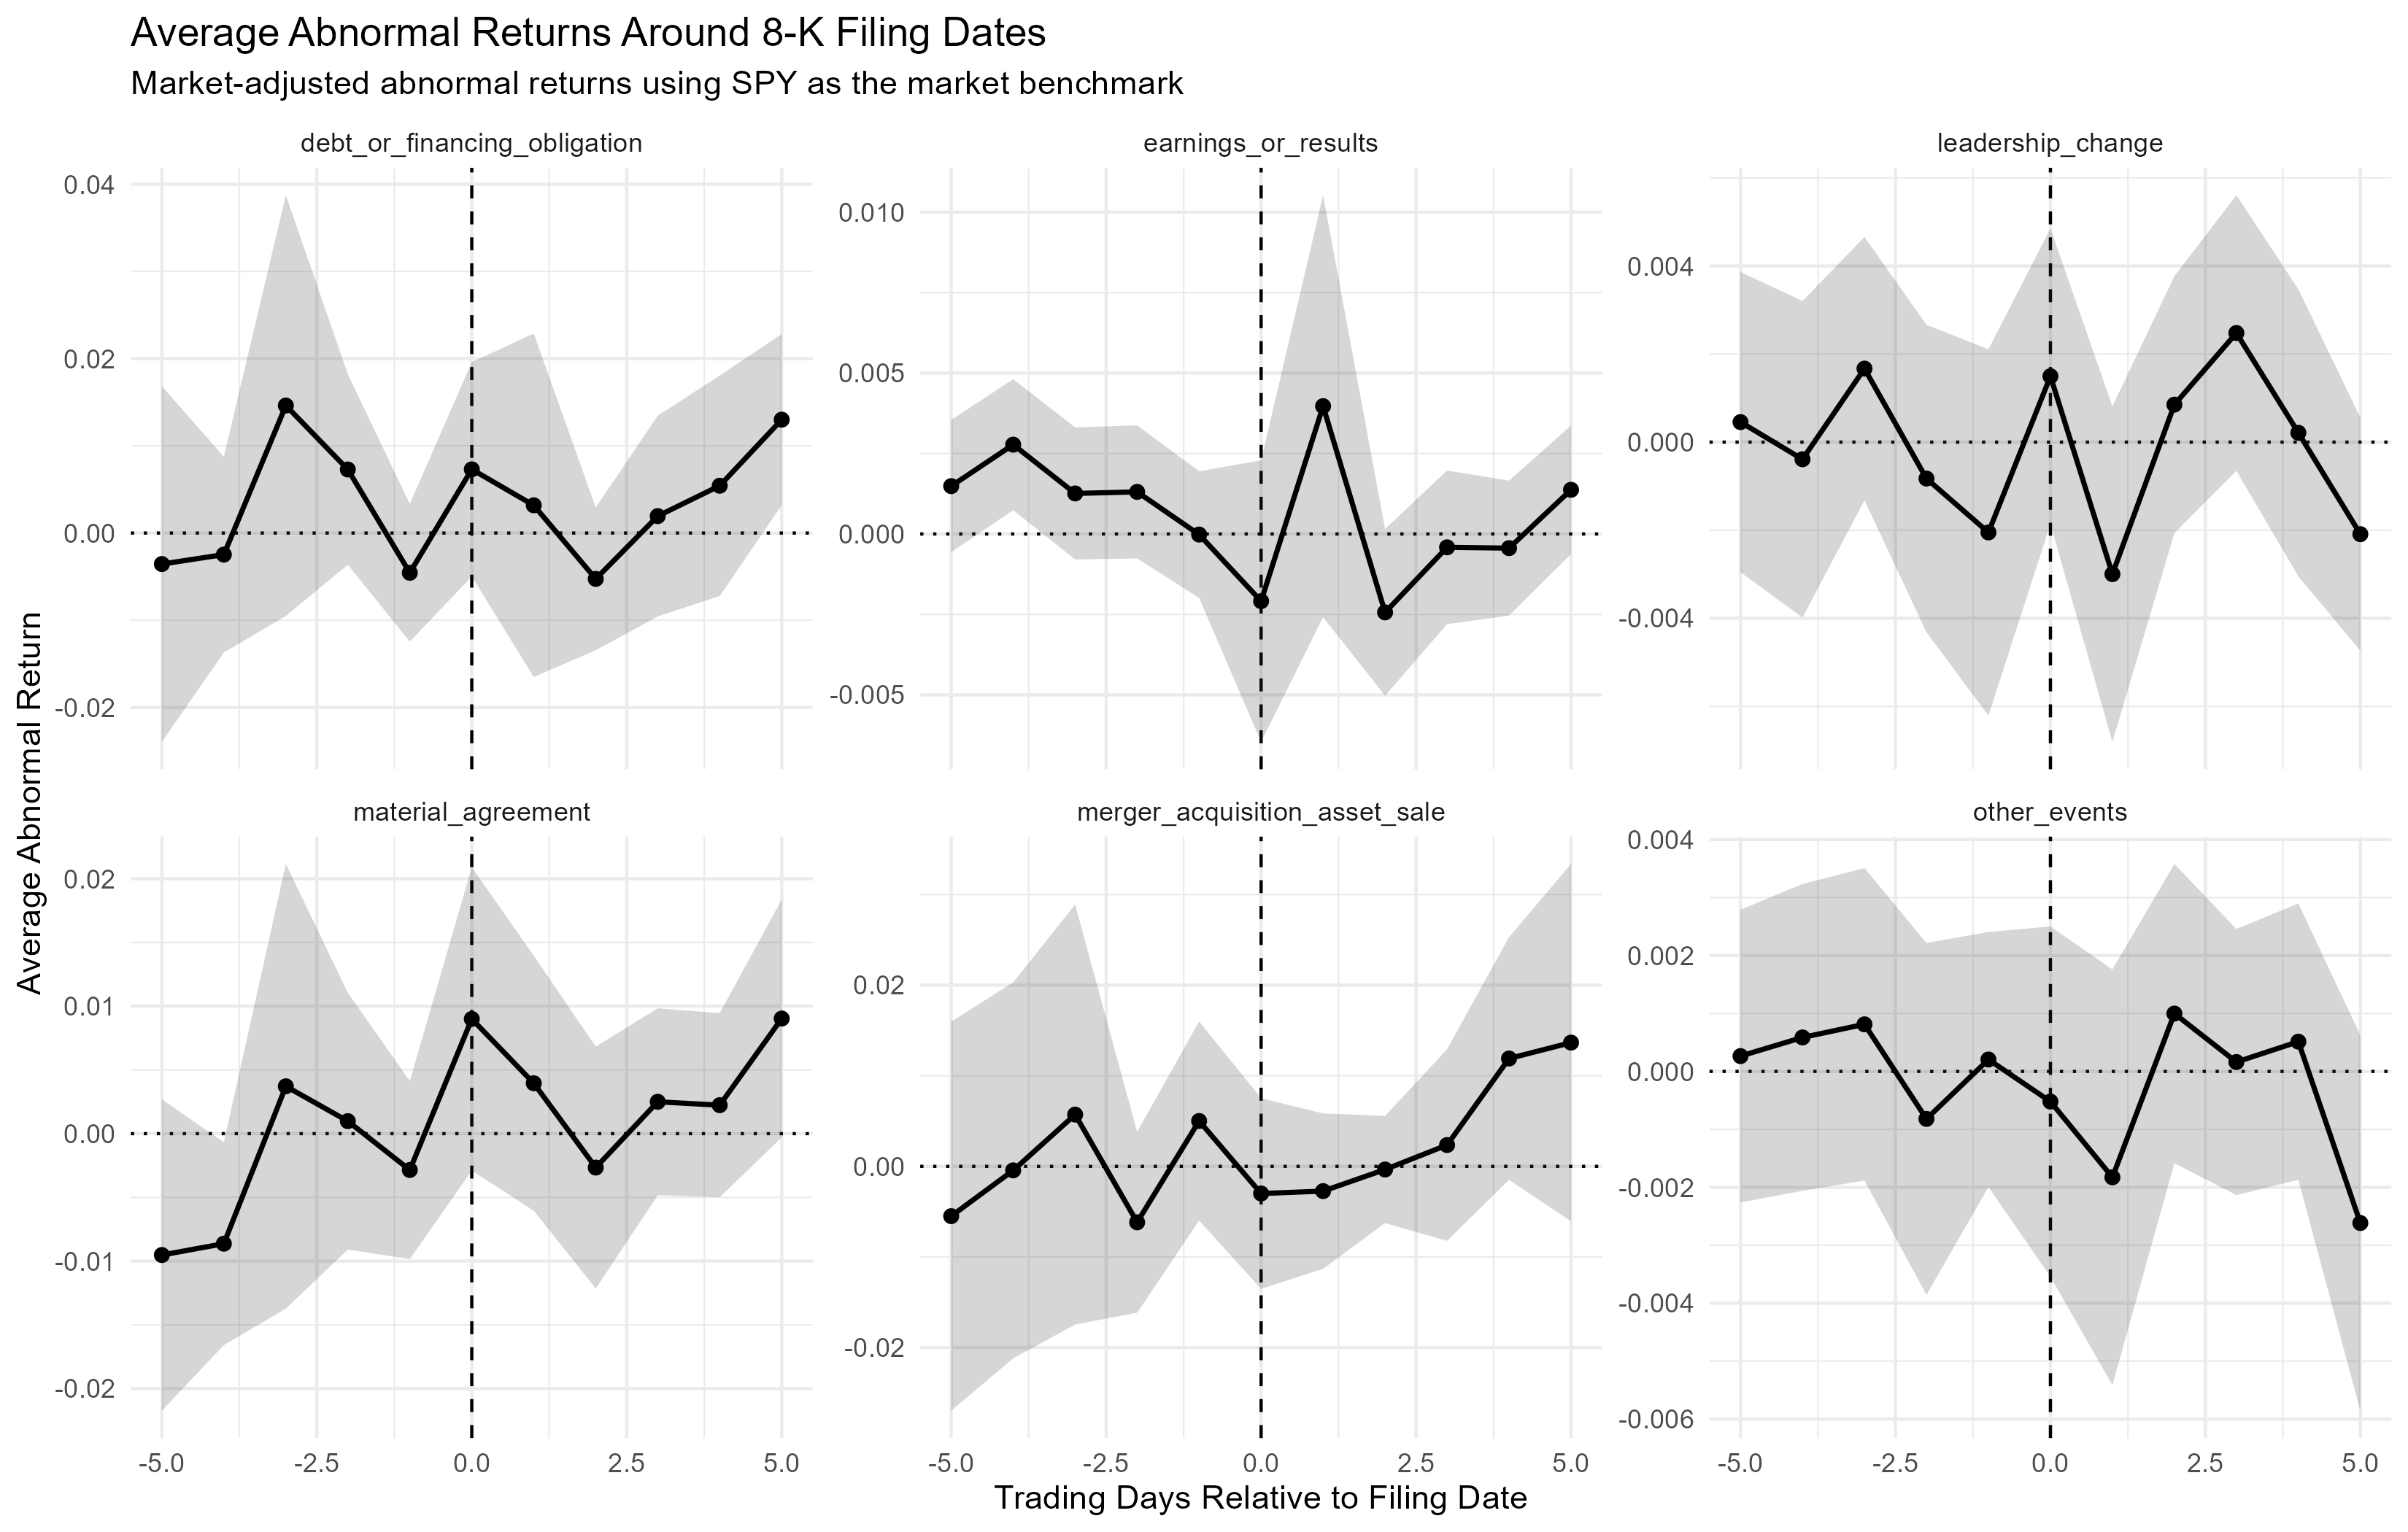
\includegraphics[width=0.95\textwidth]{../output/figures/average_abnormal_returns_by_item_group.png}
		\caption{Average Abnormal Returns Around 8-K Filing Dates}
		\label{fig:avg_ar}
	\end{figure}
	
	If markets react quickly to new public information, the largest abnormal returns should occur around event time $\tau = 0$ or $\tau = +1$. Abnormal returns before the filing date may suggest information leakage, anticipation, or that the 8-K filing date is not the first public announcement date. Abnormal returns after the filing date may suggest delayed market reaction or continued news diffusion.
	
	\subsection{Cumulative Abnormal Return Summary}
	
	Cumulative abnormal returns summarize the total abnormal performance over an event window. Table \ref{tab:car_summary} reports average and median CARs by item group.
	
	\begin{table}[H]
		\centering
		\caption{Cumulative Abnormal Returns by 8-K Item Group}
		\label{tab:car_summary}
		\resizebox{\textwidth}{!}{
			\begin{tabular}{lrrrrr}
				\toprule
				Item Group & Events & Mean CAR[-1,+1] & Median CAR[-1,+1] & Mean CAR[0,+1] & Mean CAR[0,+5] \\
				\midrule
				Earnings or results & \textit{Insert} & \textit{Insert} & \textit{Insert} & \textit{Insert} & \textit{Insert} \\
				Leadership change & \textit{Insert} & \textit{Insert} & \textit{Insert} & \textit{Insert} & \textit{Insert} \\
				Material agreement & \textit{Insert} & \textit{Insert} & \textit{Insert} & \textit{Insert} & \textit{Insert} \\
				Merger/acquisition/asset sale & \textit{Insert} & \textit{Insert} & \textit{Insert} & \textit{Insert} & \textit{Insert} \\
				Debt or financing obligation & \textit{Insert} & \textit{Insert} & \textit{Insert} & \textit{Insert} & \textit{Insert} \\
				Other events & \textit{Insert} & \textit{Insert} & \textit{Insert} & \textit{Insert} & \textit{Insert} \\
				\bottomrule
			\end{tabular}
		}
	\end{table}
	
	The CAR summary helps identify which categories are associated with larger positive or negative short-run reactions. For example, earnings-related filings may have larger absolute reactions because they contain direct information about firm performance. Leadership-change filings may have more ambiguous effects because the market's interpretation depends on whether the change is viewed as good or bad news. Material agreements and acquisitions may also vary substantially depending on the economic content of the transaction.
	
	\subsection{Sector-Level Patterns}
	
	I also summarize average CARs by GICS sector. This helps determine whether the event-study results are concentrated in particular industries.
	
	\begin{figure}[H]
		\centering
		\includegraphics[width=0.90\textwidth]{../output/figures/sector_average_car_0_p1.png}
		\caption{Average CAR[0,+1] by GICS Sector}
		\label{fig:sector_car}
	\end{figure}
	
	Sector-level differences may arise because some industries disclose different types of information more frequently, have different volatility, or face different investor expectations. For example, technology and communication services firms may experience stronger reactions to earnings-related information, while financial firms may have different sensitivities to financing-related disclosures.
	
	\subsection{Regression Results}
	
	The regression analysis compares cumulative abnormal returns across 8-K item groups. The omitted reference category is \texttt{other\_events}. Therefore, each coefficient measures the difference in average CAR between the listed item group and other events.
	
	\begin{table}[H]
		\centering
		\caption{Regression Results: CARs by 8-K Item Group}
		\label{tab:regressions}
		\resizebox{\textwidth}{!}{
			\begin{tabular}{lrrrrrr}
				\toprule
				& \multicolumn{2}{c}{CAR[-1,+1]} & \multicolumn{2}{c}{CAR[0,+1]} & \multicolumn{2}{c}{CAR[0,+5]} \\
				\cmidrule(lr){2-3}
				\cmidrule(lr){4-5}
				\cmidrule(lr){6-7}
				& Simple & FE & Simple & FE & Simple & FE \\
				\midrule
				Earnings or results & \textit{Insert} & \textit{Insert} & \textit{Insert} & \textit{Insert} & \textit{Insert} & \textit{Insert} \\
				Leadership change & \textit{Insert} & \textit{Insert} & \textit{Insert} & \textit{Insert} & \textit{Insert} & \textit{Insert} \\
				Material agreement & \textit{Insert} & \textit{Insert} & \textit{Insert} & \textit{Insert} & \textit{Insert} & \textit{Insert} \\
				Merger/acquisition/asset sale & \textit{Insert} & \textit{Insert} & \textit{Insert} & \textit{Insert} & \textit{Insert} & \textit{Insert} \\
				Debt or financing obligation & \textit{Insert} & \textit{Insert} & \textit{Insert} & \textit{Insert} & \textit{Insert} & \textit{Insert} \\
				\midrule
				Ticker fixed effects & No & Yes & No & Yes & No & Yes \\
				Year fixed effects & No & Yes & No & Yes & No & Yes \\
				Clustered SE by ticker & Yes & Yes & Yes & Yes & Yes & Yes \\
				\bottomrule
			\end{tabular}
		}
	\end{table}
	
	The fixed-effect specifications are the preferred models because they compare events within the same firm and control for common year-level shocks. A positive coefficient means that the item group is associated with a higher CAR than \texttt{other\_events}; a negative coefficient means it is associated with a lower CAR. Statistical significance should be interpreted carefully because event-study data may contain overlapping information events, unequal group sizes, and firm-specific news that is not fully controlled by the model.
	
	The coefficient plots provide a visual summary of these estimates.
	
	\begin{figure}[H]
		\centering
		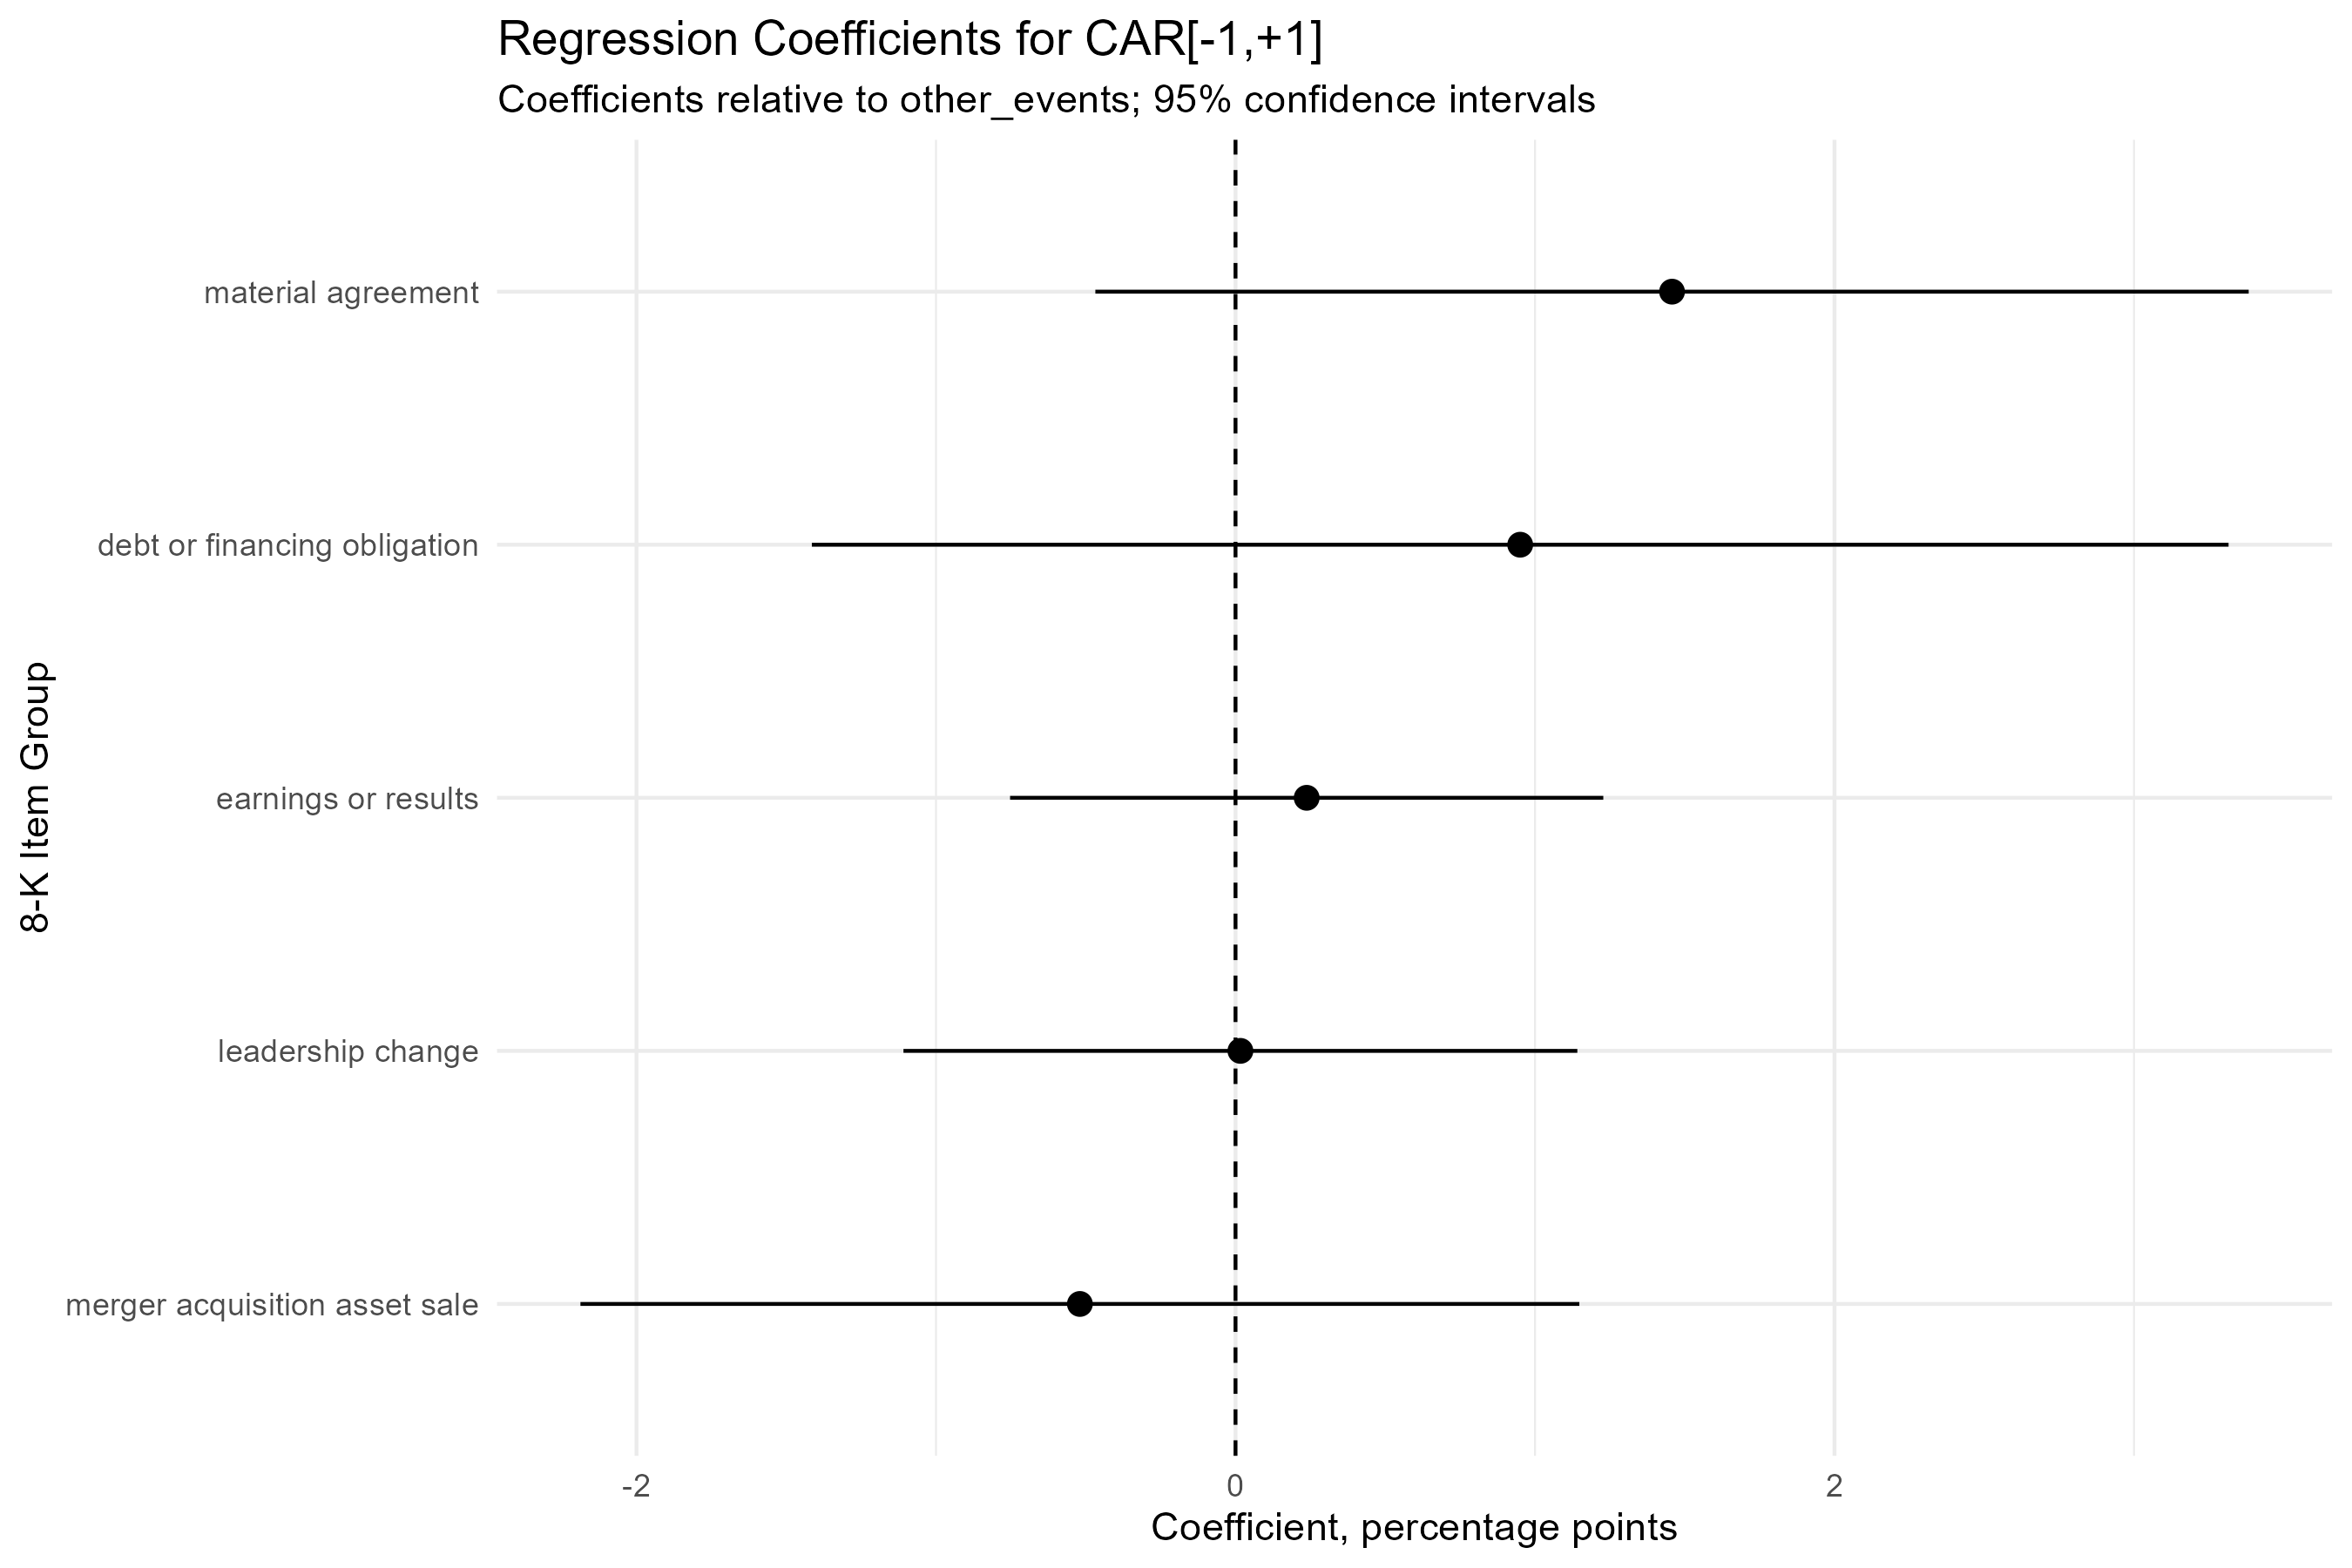
\includegraphics[width=0.90\textwidth]{../output/figures/car_coefficients_m1_p1.png}
		\caption{Regression Coefficients for CAR[-1,+1]}
		\label{fig:coef_m1_p1}
	\end{figure}
	
	\begin{figure}[H]
		\centering
		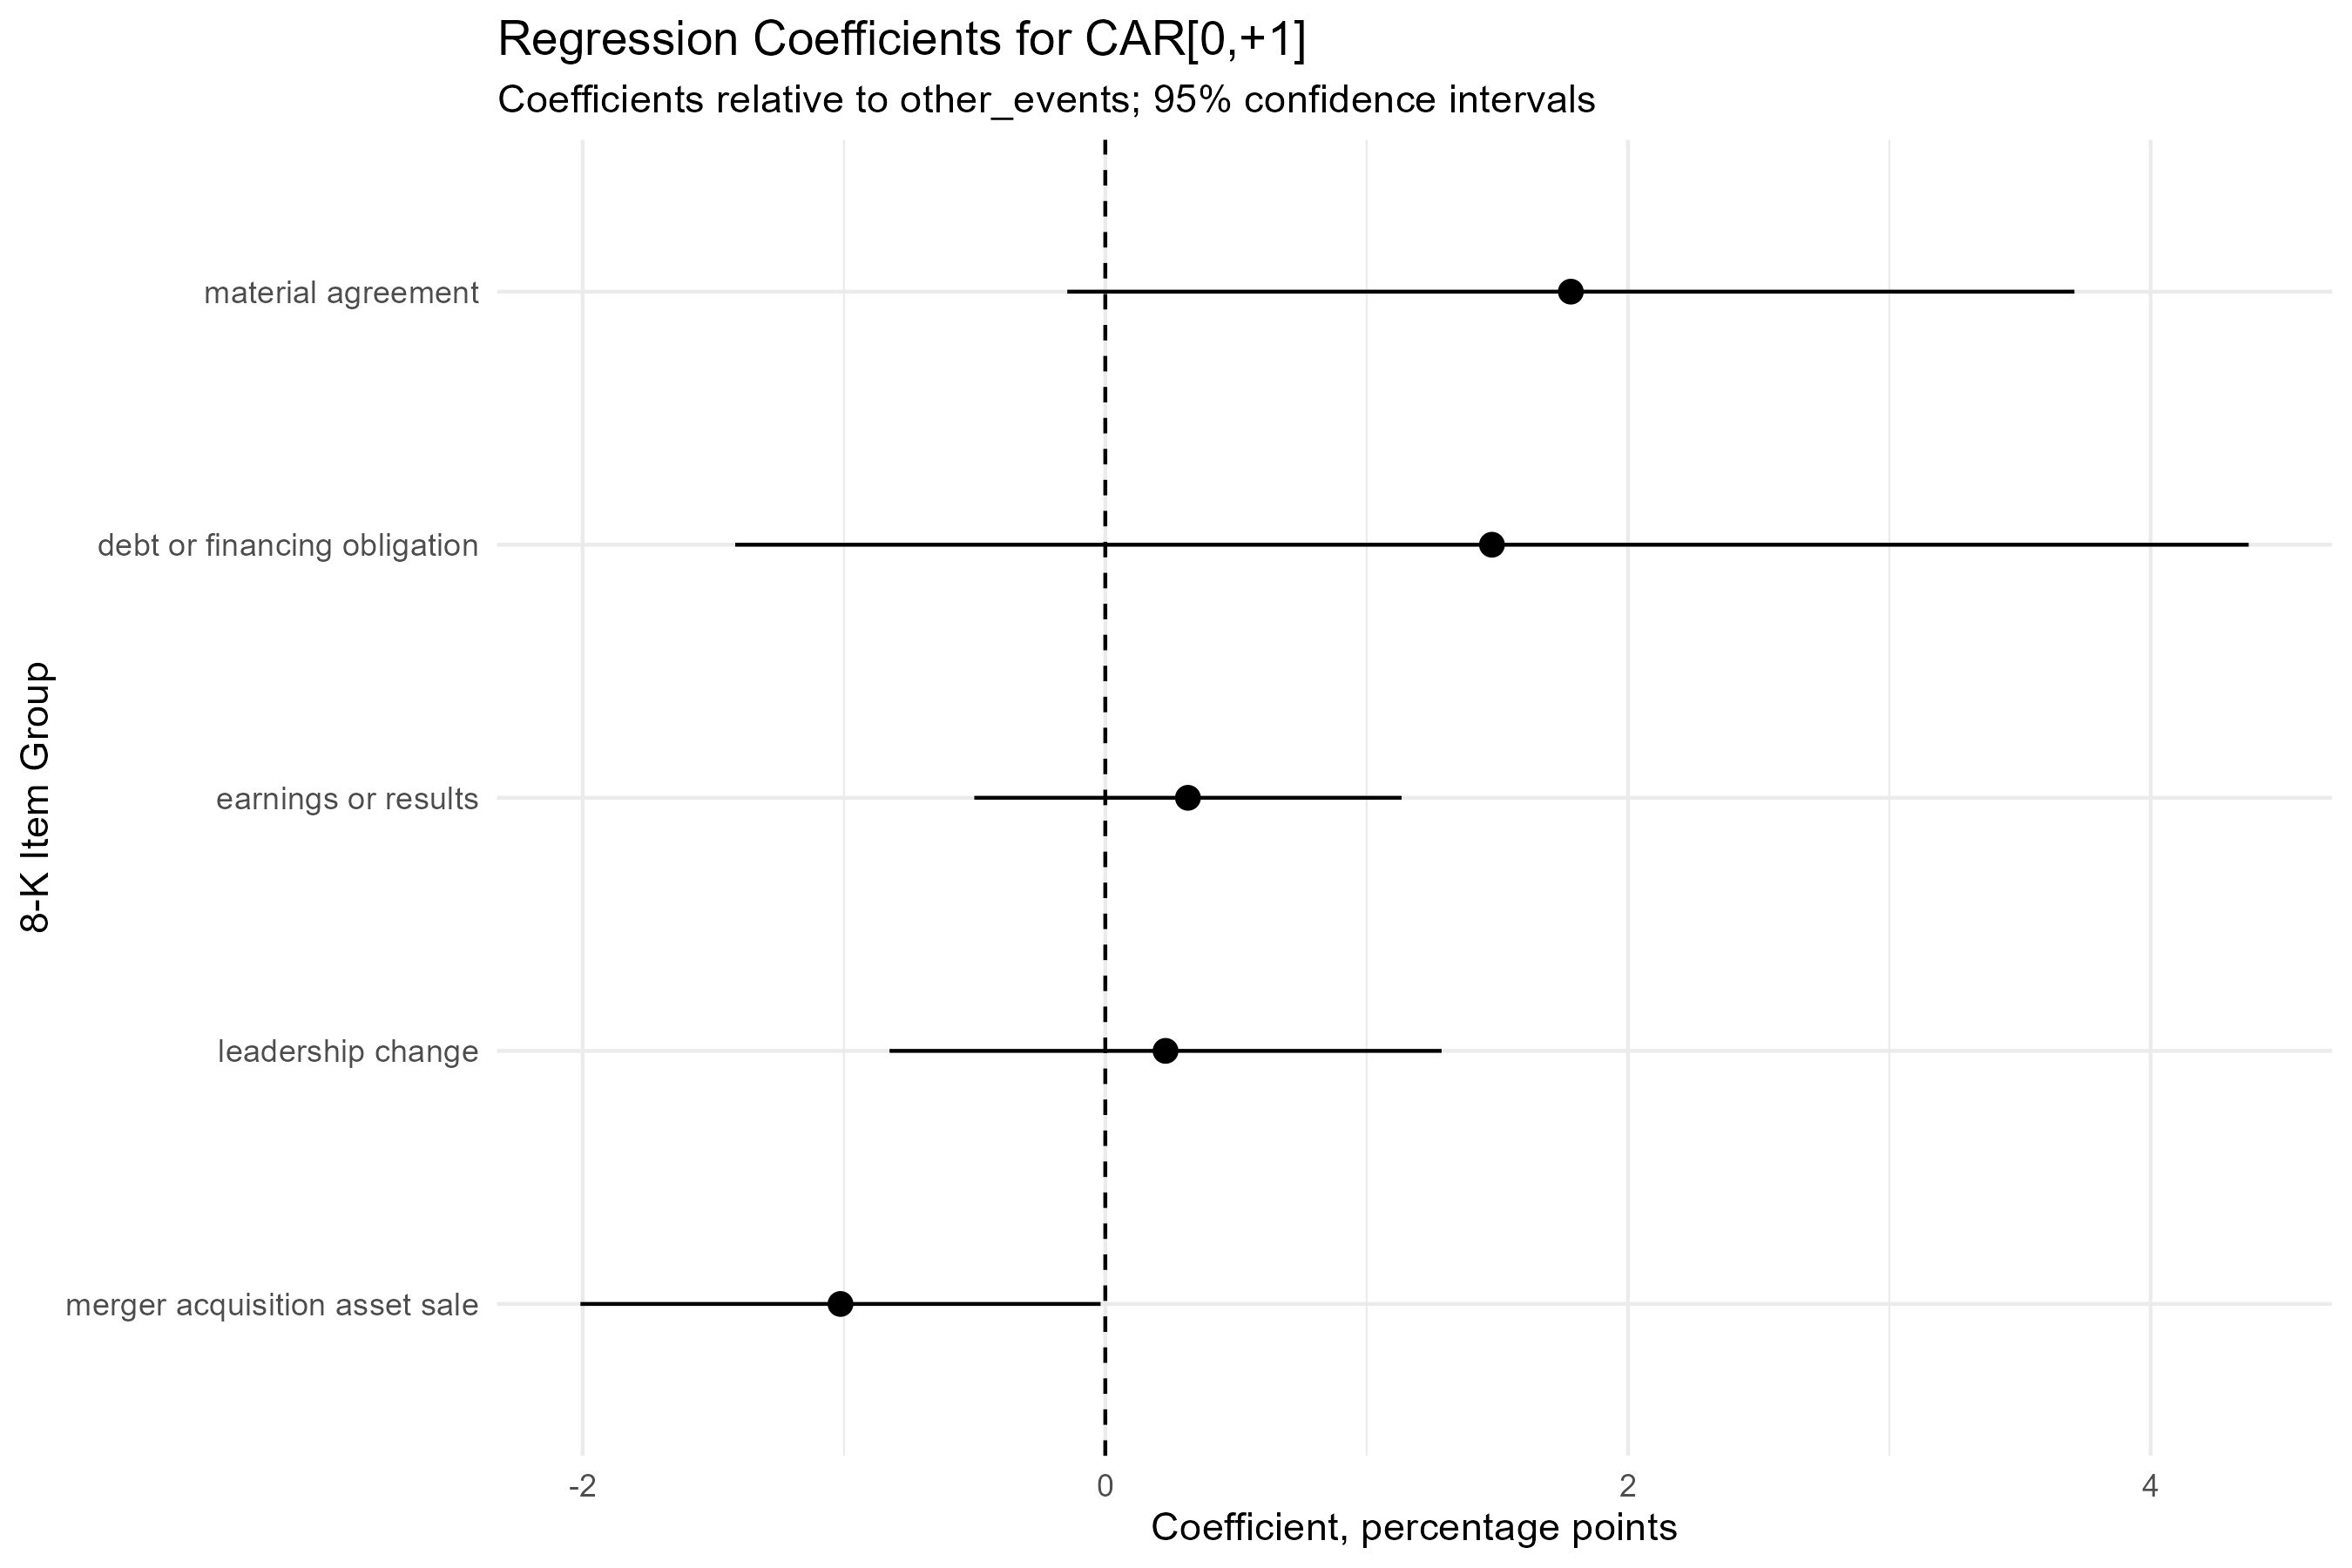
\includegraphics[width=0.90\textwidth]{../output/figures/car_coefficients_0_p1.png}
		\caption{Regression Coefficients for CAR[0,+1]}
		\label{fig:coef_0_p1}
	\end{figure}
	
	\begin{figure}[H]
		\centering
		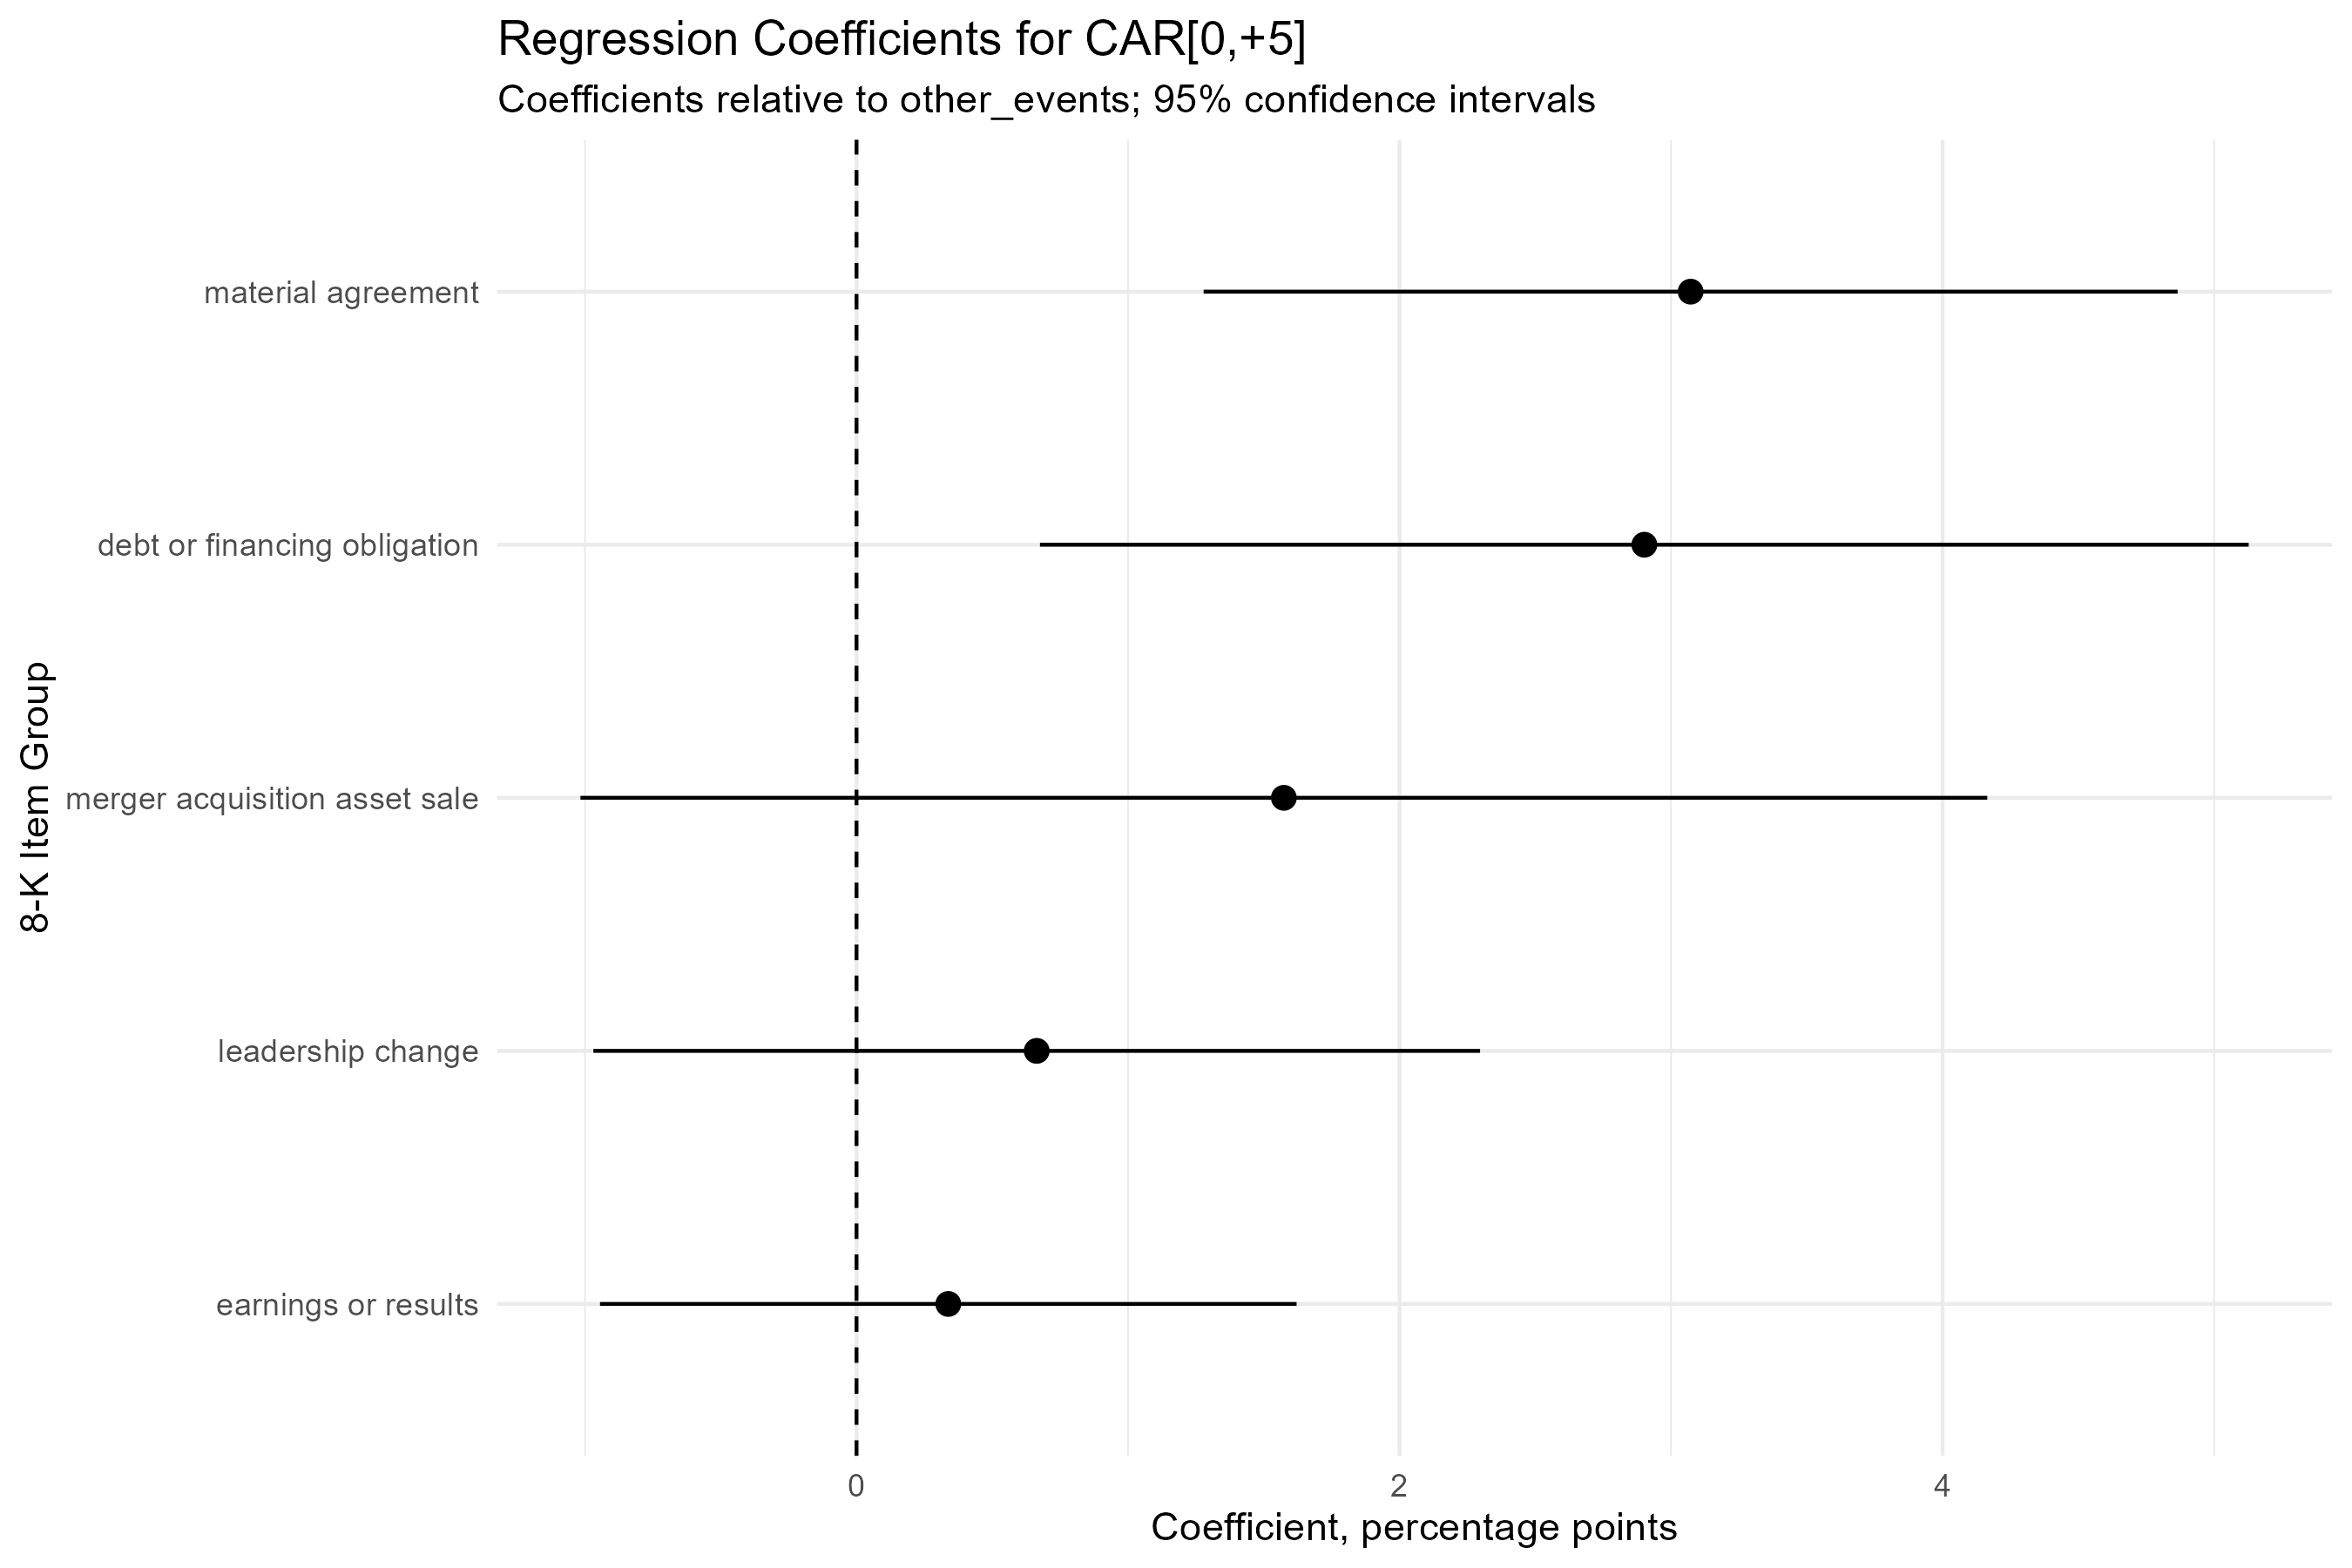
\includegraphics[width=0.90\textwidth]{../output/figures/car_coefficients_0_p5.png}
		\caption{Regression Coefficients for CAR[0,+5]}
		\label{fig:coef_0_p5}
	\end{figure}
	
	\section{Robustness Checks}
	
	Several robustness checks can strengthen the analysis.
	
	\subsection{Alternative Event Windows}
	
	The main analysis uses several CAR windows, including $[-1,+1]$, $[0,+1]$, $[0,+5]$, and $[-5,+5]$. Results should be compared across these windows. If the estimated reaction appears only in a wide window but not in a narrow window, the interpretation is less clearly tied to the filing date. If the reaction appears in $[0,+1]$, the evidence is more consistent with an immediate market response.
	
	\subsection{Excluding Overlapping Events}
	
	Some firms file multiple 8-Ks close together. If two filings occur within a few trading days of each other, it may be difficult to attribute the stock return reaction to one specific filing. A robustness check can exclude events that occur within five trading days of another 8-K filing for the same firm. This creates a cleaner but smaller sample.
	
	\subsection{Original 8-K Filings Versus Amendments}
	
	The main sample includes both 8-K and 8-K/A filings. A robustness check can estimate results using only original 8-K filings. Amendments may have different information content because they often correct, update, or supplement earlier disclosures.
	
	\subsection{Market Model Abnormal Returns}
	
	The current analysis uses market-adjusted abnormal returns:
	
	\begin{equation}
		AR_{i,t} = R_{i,t} - R_{m,t}.
	\end{equation}
	
	A more advanced robustness check is the market model. For each firm or event, estimate
	
	\begin{equation}
		R_{i,t} = \alpha_i + \beta_i R_{m,t} + \epsilon_{i,t}
	\end{equation}
	
	over a pre-event estimation window, such as $[-120,-20]$ trading days. Then compute abnormal returns as
	
	\begin{equation}
		AR_{i,t} = R_{i,t} - \left(\hat{\alpha}_i + \hat{\beta}_i R_{m,t}\right).
	\end{equation}
	
	This allows different firms to have different market betas and is more standard in event-study research. However, it also requires a longer return history and additional estimation choices.
	
	\subsection{Separating Positive and Negative News}
	
	The current item-code classification identifies the type of disclosure, not whether the news is good or bad. For example, a leadership change can be positive if investors view the new executive favorably, or negative if it signals instability. A future extension could use text analysis, earnings surprise data, or analyst forecast data to classify disclosures by news direction.
	
	\section{Limitations}
	
	This project has several important limitations.
	
	\subsection{Filing Date May Not Be the First Public Announcement Date}
	
	The event date is the SEC filing date. However, the filing date may not always be the first date on which the information became public. For example, an earnings press release may be issued before the 8-K is filed. Similarly, merger news or leadership changes may be reported by news outlets before the filing appears on EDGAR. If information reaches the market before the filing date, abnormal returns may appear before event time zero.
	
	\subsection{After-Hours and Weekend Filings}
	
	Firms can file 8-Ks after the market closes or on non-trading days. The main implementation matches filings to the next available trading day, which is more defensible than assigning weekend filings to the previous trading day. However, a more precise approach would use the SEC acceptance timestamp and market hours to distinguish filings made before the close from filings made after the close.
	
	\subsection{Yahoo Finance Data Limitations}
	
	Yahoo Finance data are convenient and free, but they are not the academic standard for event studies. Adjusted prices may differ from CRSP returns, and ticker histories can be incomplete for firms with name changes, share-class changes, mergers, or delistings. A more professional version would use CRSP through WRDS, including PERMNO identifiers and delisting returns.
	
	\subsection{Current S\&P 500 Constituents and Survivorship Bias}
	
	The sample uses current S\&P 500 constituents. Therefore, the sample excludes firms that were in the S\&P 500 during the sample period but later left the index, were acquired, or failed. This creates survivorship bias. The results should be interpreted as applying to current large-cap firms rather than to the historical S\&P 500 membership from 2018 through 2025.
	
	\subsection{CIK-Ticker Mapping Issues}
	
	SEC filings are indexed by CIK, while stock returns are indexed by ticker. Firms can change tickers, have multiple share classes, merge, spin off subsidiaries, or restructure. The project simplifies this issue by using one current ticker per CIK. This is reasonable for a beginner project but can introduce measurement error in a longer historical analysis.
	
	\subsection{Confounding Same-Day News}
	
	An 8-K filing may occur on the same day as other firm-specific news, market-wide news, analyst reports, or macroeconomic announcements. In a short event window, the hope is that unrelated confounding information is limited. However, this assumption is not guaranteed. The estimated abnormal returns should therefore be interpreted as market reactions associated with 8-K disclosure events, not as perfectly isolated causal effects of the filings themselves.
	
	\section{Conclusion}
	
	This project builds a reproducible event-study pipeline to estimate short-run stock-market reactions around SEC 8-K filings. The analysis combines SEC EDGAR filing metadata with daily stock returns, parses 8-K item codes, classifies corporate events, constructs trading-day event windows, estimates market-adjusted abnormal returns, computes cumulative abnormal returns, and compares reactions across event types using regression models.
	
	The project demonstrates several important empirical finance skills. First, it shows how to obtain and clean SEC filing data. Second, it shows how to merge disclosure events to financial market data using firm identifiers. Third, it implements the basic logic of an event study, including abnormal returns and cumulative abnormal returns. Fourth, it uses regression models with fixed effects and clustered standard errors to compare event categories. Finally, it produces tables and figures suitable for a research report or GitHub portfolio.
	
	The main empirical object is the cumulative abnormal return around an 8-K filing. The results should be interpreted as evidence on short-run market reactions associated with different types of corporate disclosures. Because the event date is the filing date rather than necessarily the first public announcement date, and because other news may occur near the same time, the analysis should not be interpreted as a perfect causal estimate. Nevertheless, the project provides a strong foundation for learning empirical finance, R programming, financial data cleaning, and event-study methodology.
	
	Future extensions could improve the project by using CRSP returns, historical S\&P 500 membership, more precise after-hours filing treatment, market-model abnormal returns, overlapping-event filters, and text-based classification of positive versus negative news. These additions would make the project closer to a professional academic event study.
	
\end{document}
